%=============================================================================
% ..... THIS IS chapter{G.726: The ITU-T ADPCM algorithm } .....
% ... Revision:
% Ago.1992 - M.Sheriff suggestions
% Ago.1992 - Some stilish changes
% Sep.1992 - M.Sheriff further suggestions
% Jan.1995 - Some changes in the call for the routines
% Oct.1995 - Replaced some references to G.721 to G.726
% Jan.1996 - Peter Kroon revision incorporated
% Feb.2000 - Convergence towards STL2000
% Feb.2001 - Edits in example section
%=============================================================================
\chapter{G.726: The ITU-T ADPCM algorithm at 40, 32, 24, and 16 kbit/s}
%=============================================================================

In 1982, a group was established by the then CCITT Study Group XVIII
to study the standardization of a speech coding technique that could
reduce the 64 kbit/s rate used in digital links, as per
Recommendation ITU-T G.711 (see related Chapter), by half while
maintaining the same voice quality.

After considering contributions received from several organizations, there was
a general feeling that the ADPCM {\em (Adaptive Differential Pulse Code
Modulation)} technique could provide a good quality coder. This process
of finalizing an algorithm took 18 months of development and objective
and subjective testings, to culminate in an ITU Recommendation,
published in October, 1984, and available in the Red Book series as
Recommendation ITU-T G.721.

Meanwhile, problems were found with the G.721 algorithm of 1984
regarding voice-band data signals modulated using the Frequency Shift
Keying (FSK) technique, and changes had to be done to the algorithm.
These changes were approved in 1986 and published in the next series of
Recommendations of the CCITT, the Blue Book series, superseeding the
Red Book version of the G.721. This is why a note in the Blue Book
G.721 warns the user that the bit stream of coded speech from this
version is incompatible with the old one. Also in that Study Period
(1985-1988), a need for other rates was identified, and a new
Recommendation, ITU-T G.723, was approved to extend the bitrate to 24 and 40
kbit/s.

In the Study Period of 1989--1992, these two Recommendations have been
joined into a single one, keeping full compatibility with the former
ones, and adding a lower rate of 16 kbit/s. This new Recommendation was
named ITU-T G.726, and the former ITU-T G.721 and G.723 have been replaced.

The current version of the STL includes a G.726 implementation. In the
section to follow, the operation of the G.726 algorithm is described
only for the 32 kbit/s bit rate. A complete description of the G.726
algorithm can be found in \cite{G.726}. Other analyses of the
algorithm, besides some based on the Red Book version, can be found in
several studies \cite{ADPCM-theor,ADPCM-over,ADPCM-Tech-Report}.

Despite the change in numbering, the ITU-T ADPCM algorithm for speech
coding at 32 kbit/s, the term ``G.721 algorithm'' has been retained
for simplicity of the text, although a more formal reference
should be {\em ``G.726 at 32 kbit/s''}.

\section{Description of the 32 kbit/s ADPCM}

The basic idea behind the G.721 coder is to code into 4-bit samples the
input speech-band signals, sampled at 8 kHz and represented by the
8-bit of G.711 A or $\mu$ law samples. The decoder just implements the
reverse procedure.

The ADPCM algorithm of the G.721 exploits the predictability of the
speech signals. Therefore, an adaptive predictor is used to compute the
difference signal $d(k)$ (based on the expanded input log-pcm sample
$s(k)$), which is then quantized by an adaptive quantizer using 4 bits.
These bits are sent to the decoder and then fed into an inverse
quantizer. The difference signal is used to calculate the reconstructed
signal, $s_r(k)$, which is compressed (A- or $\mu$-law) and output from
the decoder ($s_d(k)$).

From this description, one could ask the following:

\rulex{5mm}\begin{minipage}{140mm}
 $\bullet$ If only the quantized signal is transmitted, how can the
        decoder reconstruct  \rulex{2.5ex} the signal?

 $\bullet$ How can one assure estability of the predictor?

 $\bullet$ Will this bitrate reduction degrade the voice quality?
\end{minipage}

These and others have already been considered in the design of the
G.721, and many blocks of the algorithm are made to assure a good
behaviour. For example, one possibility in this backward approach for
adaptation is to have encoder and decoder starting from the same point,
which is accomplished by reseting key variables to a known state
(useful for implementation verification). Leak factors have been
introduced to ensure that the algorithm will always converge,
independently of the initial state. To avoid instabilities, some
parameters had their range limited. To provide some insight in the
building blocks of the G.721 algorithm, a short description of each of
them is given \cite{G.726,ADPCM-over}.


\subsection{PCM format conversion}

The input signal $s(k)$, in either A- or $\mu$-law format, must be
converted into linear samples. This expansion is accomplished using the
same algorithm in G.711 \cite{G.711}, but converting from signed
magnitude to 14-bit two's complement samples.


\subsection{Difference Signal Computation}

This block simply calculates the difference between the (expanded) input signal and the estimated signal:
\[
      d(k) = s_l(k) - s_e(k)
\]


\subsection{Adaptive Quantizer}

A 15-level, non-uniform adaptive quantizer is used to quantize the
difference signal. Before the quantization, this signal is converted to
a logarithmic representation\footnote{\SF Remember that to multiply
samples in the linear domain one may add in the logarithmic one. Using
efficient log and exponentiation algorithms (as done here), this turns
out to be very advantageous.} and scaled by a factor ($y(k)$), that is
computed in the scale factor adaptation block (see below).

The output of this block is $I(k)$, and it is used twice; first, is
the ADPCM coded ({\em quantized}) sample; second, is the input to the
backward part of the G.721 algorithm, to provide information for
quantization of the next samples. One relevant point to notice here
is that the backward adaptation is done using the quantized sample.
If one starts the decoder from this very point, one will find
identical behaviour. That is why only the  quantized samples are
needed in the decoder (i.e., no side information).


\subsection{Inverse Adaptive Quantizer}

The inverse adaptive quantizer takes the signal $I(k)$ and converts it
back to the linear domain, generating a quantized version of the
difference signal, $d_q(k)$. This is the input to the adaptive
predictor, such that the estimated signal is based on a quantized
version of the difference signal, instead of on the unquantized
(original) one.


\subsection{Quantizer Scale Factor Adaptation}

This block computes $y(k)$, the factor used in the adaptive quantizer
and inverse quantizer for domain conversion. As input, this block
needs $I(k)$, but also $a_l(k)$, the adaptation speed control
parameter. The reason for the latter is that the scaling algorithm
has two modes ({\em bimodal adaptation}), one fast, another slow.
This has been done to accomodate signals that in nature produce
difference signals with large fluctuations (e.g. speech) and small
fluctuations (e.g. tones and voice-band data), respectively.

This block computes two scale factor (fast, $y_u(k)$, and slow,
$y_l(k)$) based on $I(k)$, which combined using $a_l(k)$ produce
$y(k)$.


\subsection{Adaptation Speed Control}

This block evaluates the parameter $a_l(k)$, which can be seen as a
{\em proportion} of the speed (fast or slow) of the input signal, and
is in the range $[0,1]$. If 0, the data are considered to be {\em
slowly} varying; if 1, they are considered to be {\em fast}
varying.

To accomplish this, two measures of the average magnitude of $I(k)$ are
computed ($d_{ms}(k)$ and $d_{ml}(k)$). These, in conjunction with
delayed tone detect and transition detect flags ($t_d(k)$ and $t_r(k)$,
calculated in the Tone Transition and Detector block), are used to
evaluate $a_p(k)$, whose delayed version ($a_p(k-1)$) is used in the
definition of $a_l(k)$, limiting the range to $[0,1]$\footnote{\SF This
limitation delays the start of a fast to slow transition until the
average magnitude of $I(k)$ remains constant for some time; acting so,
premature transitions for pulsed input signals, such as switched
carrier voiceband data, are avoided.}.

An analysis of $a_p(k)$ gives insight on the nature of the signal: if
around the value of 2, this means that the average magnitude of $I(k)$
is changing, or that a tone has been detected, or that it is idle
channel noise; on the other side, if near 0, the average magnitude of
$I(k)$ remains relatively constant.


\subsection{Adaptive Predictor and Reconstructed Signal Calculator}

The adaptive predictor has as its main function to compute the signal
estimate based on the quantized difference signal, $d_q(k)$. It has 6
zeroes and 2 poles, structure that covers well the kind of input
signals expected for the algorithm. With these coefficients, and past
values of $d_q(k)$ and $s_e(k)$, the updated value for the signal
estimate $s_e(k)$ is computed.

The two sets of coefficients (one for the pole section, $a_i(k),
i=1..2$, other for the zero section, $b_i(k), i=1..6$) are updated
using a simplified gradient algorithm. At this point, since a situation
in which the poles cause instability may arise, the two pole
coefficients $a_i$ have their ranges limited. In addition, if a
transition from partial band signal is detected (signaled by $t_r(k)$),
the predictor is reset (all coefficients are set to 0), remaining
disabled until $t_r$ comes back to zero\footnote{\SF Note that when
this happens, the quantizer is forced into the fast mode of
adaptation.}.

The reconstructed signal $s_r(k)$ is calculated using the signal
estimate $s_e(k)$ and the quantized difference signal $d_q(k)$.


\subsection{Tone Transition and Detector}

This block is one of the changes from the Red Book version. It was
added to improve algorithm performance for signals originating from
FSK modems operating in the character mode.  First, it checks if the
signal has partial band (e.g., a tone) by looking at the predictor
coefficient $a_2(k)$, that defines the signal $t_d(k)$.  Second, a
transition from partial band signal indicator $t_r(k)$ is set, such
that predictor coefficients can be set to 0 and the quantizer can be
forced into the fast mode of operation.

\subsection{Output PCM Format Conversion}

This block is unique to the decoder. Its sole function is to compress
the reconstructed signal $s_r(k)$, which is in linear PCM format, using
A or $\mu$ law, and is a complement of the PCM format conversion
block.


\subsection{Synchronous Coding Adjustment}

This block is also unique to the decoder. It has been devised in order
to prevent cumulative distortions occuring on synchronous tandem
codings (ADPCM--\-PCM--\-ADPCM, etc., in purely digital connections, i.e.,
with no intermediate analog conversions), provided that:

\rulex{5mm} $\bullet$ \parbox[t]{140mm}{
               the transmission of the ADPCM and the intermediate PCM are
               error-free, and }

\rulex{5mm} $\bullet$ \parbox[t]{140mm}{
               the ADPCM and the intermediate PCM are not disturbed by digital
               signal processing devices.}

\subsection{Extension for linear input and output signals}

An extension of the G.726 algorithm was carried out in 1994 to include, as
an option, linear input and output signals. The specification for such linear
interface is given in its Annex A \cite{G.726:LinearIO}.

This extension bypasses the PCM format conversion block for linear input
signals, and both the Output PCM Format Conversion and the Synchronous
Coding Adjustment blocks, for linear output signals. These linear versions
of the input and output signals are 14-bit, 2's complement samples.

The effect of removing the PCM encoding and decoding is to decrease the
coding degradation by 0.6 to 1 qdu, depending on the network configuration
considered (presence or absence of a G.712 filtering).

Currently, this extension has not been incorporated in the STL.


\section{ITU-T STL G.726 Implementation}

The STL implementation of the G.726 algorithm can be found
in module {\tt g726.c}, with prototypes in {\tt g726.h}.

Originally in Fortran (VAX Fortran-77), the source was translated by means
of the public-domain code converter {\em f2c} \cite{f2c}. This explain why
the code makes extensive use of passage of parameters by reference, rather
than by value, and why many functions, that could be implemented as macros
(using the C pre-processor directive {\tt \#define}), are routines, and as
well as all routines return {\tt void}.

The problem of storing the state variables was solved by defining a
structure containing all the necessary variables, defining a new type
called {\tt G726\_state}. By means of this approach, several streams
may be processed in parallel, provided that one structure is assigned
(and that one call to the encoding/decoding routines is done) for
each data stream (this can be advantageous for machines with support
for parallel processing). The G726 state variable  structure has the
following fields (all are {\tt short}, except {\em ylp},  which is
{\tt long}):

\begin{quote} \normalsize
 {\em sr0} \hfill \pbox{120mm}{ Reconstructed signal with delay 0}\\
 {\em sr1} \hfill \pbox{120mm}{ Reconstructed signal with delay 1}\\
 {\em a1r} \hfill \pbox{120mm}{ Delayed 2nd-order predictor coefficient 1}\\
 {\em a2r} \hfill \pbox{120mm}{ Delayed 2nd-order predictor coefficient 2}\\
 {\em b1r} \hfill \pbox{120mm}{ Delayed 6th-order predictor coefficient 1}\\
 {\em b2r} \hfill \pbox{120mm}{ Delayed 6th-order predictor coefficient 2}\\
 {\em b3r} \hfill \pbox{120mm}{ Delayed 6th-order predictor coefficient 3}\\
 {\em b4r} \hfill \pbox{120mm}{ Delayed 6th-order predictor coefficient 4}\\
 {\em b5r} \hfill \pbox{120mm}{ Delayed 6th-order predictor coefficient 5}\\
 {\em b6r} \hfill \pbox{120mm}{ Delayed 6th-order predictor coefficient 6}\\
 {\em dq0} \hfill \pbox{120mm}{ Quantized difference signal with delay 0}\\
 {\em dq1} \hfill \pbox{120mm}{ Quantized difference signal with delay 1}\\
 {\em dq2} \hfill \pbox{120mm}{ Quantized difference signal with delay 2}\\
 {\em dq3} \hfill \pbox{120mm}{ Quantized difference signal with delay 3}\\
 {\em dq4} \hfill \pbox{120mm}{ Quantized difference signal with delay 4}\\
 {\em dq5} \hfill \pbox{120mm}{ Quantized difference signal with delay 5}\\
 {\em dmsp} \hfill \pbox{120mm}{ Short term average of the $F(I)$ sequence }\\
 {\em dmlp} \hfill \pbox{120mm}{ Long term average of the $F(I)$ sequence}\\
 {\em apr} \hfill \pbox{120mm}{ Triggered unlimited speed control parameter}\\
 {\em yup} \hfill \pbox{120mm}{ Fast quantizer scale factor }\\
 {\em tdr} \hfill \pbox{120mm}{ Triggered tone detector }\\
 {\em pk0} \hfill \pbox{120mm}{ Sign of dq+sez with delay 0}\\
 {\em pk1} \hfill \pbox{120mm}{ Sign of dq+sez with delay 1}\\
 {\em ylp} \hfill \pbox{120mm}{ Slow quantizer scale factor }\\
\end{quote}


The encoding function is {\tt G726\_encode}, and the decoding function
is {\tt G726\_decode}. There are 41 other routines that, grouped in
individual calls inside the encoder and decoder, implement the
algorithm. Therefore, none of these 41 routines are expected to be
accessed by the user, and only the two main ones.

In the following part a summary of calls to both functions is found.

\subsection{{\tt G726\_encode}}

{\bf Syntax: }

{\tt
\#include "g726.h"\\
void G726\_encode
         (\ttpbox{110mm}{
            short {\em *inp\_buf}, short {\em *out\_buf}, long {\em smpno},
             char  {\em *law}, short {\em rate}, short {\em reset},
             G726\_state {\em *state})
         }
}

%------------------ Begin of parallel-form IIR filter --------------------
\begin{figure}
  \begin{center}
    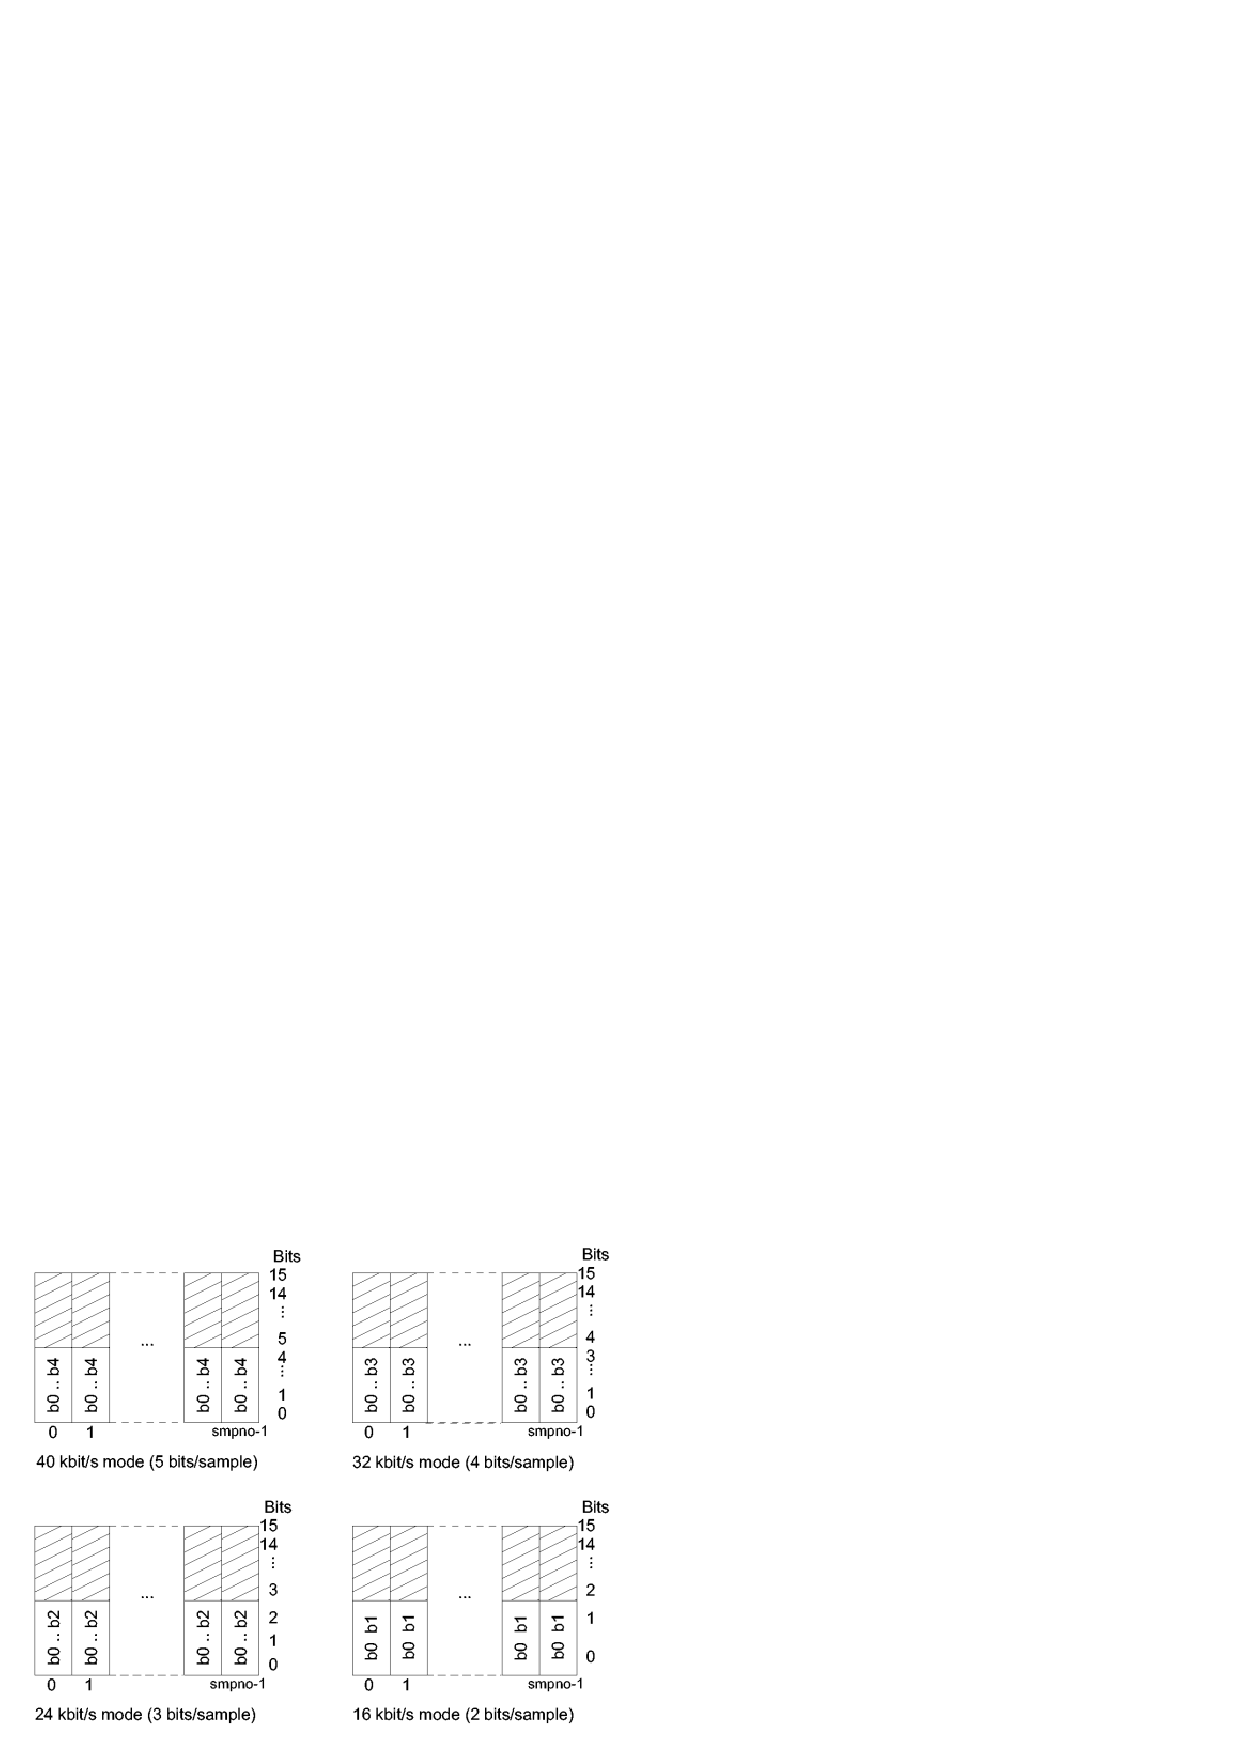
\includegraphics{bs-g726}
  \end{center}
  \caption{\SF Packing of G.726-encoded signals (right-aligned,
               parallel format).\label{G726-bs}}
\end{figure}
%------------------ End of IIR filter -----------------------------------

{\bf Prototype: }    g726.h

{\bf Description: }

        Simulation of the ITU-T G.726 ADPCM encoder. Takes the A or
        $\mu$ law input array of shorts {\em inp\_buf} (16 bit,
        right-justified, without sign extension) with {\em smpno}
        samples, and saves the encoded samples in the array of shorts
        {\em out\_buf}, with the same number of samples and
        right-justified. An example of the sample packing for the
        G.726 encoded bitstream is shown in figure \ref{G726-bs}.

        The state variables are saved in the structure {\em state}, and the
        reset can be stablished by making {\em reset} equal to 1. The law
        is A if {\em law}=={\tt '1'}, and mu law if {\em law}=={\tt
        '0'}.

{\bf Variables: }
\begin{Descr}{\DescrLen}
\item[\pbox{20mm}{\em inp\_buf}] %\rulex{1mm}\\
               Is the input samples' buffer; each {\tt short} sample
               shall contain right-justified 8-bit wide valid A or $\mu$
               law samples.

\item[\pbox{20mm}{\em out\_buf}] %\rulex{1mm}\\
               Is the output samples' buffer; each {\tt short} sample
               will contain right-justified 2-, 3-, 4-, or 5-bit wide G.726
               ADPCM samples, depending on the rate used.

\item[\pbox{20mm}{\em smpno}] %\rulex{1mm}\\
               Is the number of samples in inp\_buf.

\item[\pbox{20mm}{\em law}] %\rulex{1mm}\\
               Is a char indicating if the law for the input samples is A
               ({\tt '1'}) or $\mu$ ({\tt '0'}). See note below.

\item[\pbox{20mm}{\em rate}] %\rulex{1mm}\\
               Is a short indicating the number of bits per sample to used by
               the algorithm: 5, 4, 3, or 2.

\item[\pbox{20mm}{\em reset}] %\rulex{1mm}\\
               Is the reset flag (see note below):\\
               $\bullet$ {\em 1}: reset is to be applied in the variables;\\
               $\bullet$ {\em 0}: processing is carried out without
               setting state variables to the reset state. \\
               Please note that this should normally be
               done only in the first call to the routine in processing a
               sample stream.

\item[\pbox{20mm}{\em state}] %\rulex{1mm}\\
               The state variable structure; all the variables here are for
               internal use of the G.726 algorithm, and should not be
               changed by the user. Fields of this structure are described
               above.
\end{Descr}

{\bf Note:} \hfill \pbox{145mm}{
               Please note the difference between {\em reset} and {\em
               law}: {\em reset} must be either 1 (0x01) or 0 (0x00), not
               `1' (0x31) or `0' (0x30), while {\em law} is exactly
               the opposite.
             }\\

{\bf Return value: }        None.


\subsection{{\tt G726\_decode}}

{\bf Syntax: }

{\tt
\#include "g726.h"\\
void G726\_decode
         (\ttpbox{110mm}{
             short {\em *inp\_buf}, short {\em *out\_buf}, long {\em smpno},
             char  {\em *law}, short {\em rate}, short {\em reset},
             G726\_state {\em *state})
         }
}

{\bf Prototype: }    g726.h

{\bf Description: }

        Simulation of the ITU-T G.726 ADPCM decoder. Takes
        the ADPCM input array of shorts {\em inp\_buf} (16 bit, right-
        justified, without sign extension) of length {\em smpno}, and
        saves the decoded samples (A or $\mu$ law) in the array of
        shorts {\em out\_buf}, with the same number of samples and
        right-justified.

        The state variables are saved in the structure {\em state}, and the
        reset can be stablished by making {\em reset} equal to 1. The law
        is A if {\em law}=={\tt '1'}, and mu law if {\em law}=={\tt
        '0'}.

{\bf Variables: }
\begin{Descr}{\DescrLen}
\item[\pbox{20mm}{\em inp\_buf}] %\rulex{1mm}\\
               Is the input samples' buffer; each {\tt short} sample
               will contain right-justified 2-, 3-, 4-, or 5-bit wide
               G.726 ADPCM samples.

\item[\pbox{20mm}{\em out\_buf}] %\rulex{1mm}\\
               Is the output samples' buffer; each {\tt short} sample
               shall contain right-justified 8-bit wide valid A or $\mu$
               law samples.

\item[\pbox{20mm}{\em smpno}] %\rulex{1mm}\\
               Is the number of samples in inp\_buf.

\item[\pbox{20mm}{\em law}] %\rulex{1mm}\\
               Is a char indicating if the law for the input samples is A
               ({\tt '1'}) or $\mu$ ({\tt '0'}). See note below.

\item[\pbox{20mm}{\em rate}] %\rulex{1mm}\\
               Is a short indicating the number of bits per sample to used by
               the algorithm: 5, 4, 3, or 2.

\item[\pbox{20mm}{\em reset}] %\rulex{1mm}\\
               Is the reset flag (see note below):\\
               $\bullet$ {\em 1}: reset is to be applied in the variables;\\
               $\bullet$ {\em 0}: processing done without setting state
               variables to reset state. \\
               Please note that this should normally be
               done only in the first call to the routine in processing a
               sample stream.

\item[\pbox{20mm}{\em state}] %\rulex{1mm}\\
               The state variable structure; all the variables here are for
               internal use of the G.721 algorithm, and should not be
               changed by the user. Fields of this structure are described
               above.
\end{Descr}

{\bf Note:} \hfill \pbox{145mm}{
               Please note the difference between {\em reset} and {\em
               law}: {\em reset} must be either 1 (0x01) or 0 (0x00), not
               `1' (0x31) or `0' (0x30), while {\em law} is exactly
               the opposite.
             }\\

{\bf Return value: }        None.


%-.-.-.-.-.-.-.-.-.-.-.-.-.-.-.-.-.-.-.-.-.-.-.-.-.-.-.-.-.-.-.
\section{Portability and compliance} \label{G.726-Port}

Code testing has been done using the reset test sequences for 40, 32,
24, and 16 kbit/s provided in the G.726 test sequence diskettes
(available from the ITU sales department). Other tests were also done
with speech files for the 32 kbit/s mode, comparing with reference
implementations, most noticeably the one from AT\&T Bell Laboratories,
which is the original implementation. Both test approaches generated
100\% compatibility of this implementation with the G.726.
\footnote{\SF The problem with the A-law 40 kbit/s test vector
{\tt ri40fa.o} present in the STL96 has been solved in the STL2000.}

The portability of the STL G.726 encoding function has been tested by
feeding the routine with the reset test sequences of the G.726 test
sequences diskettes (available from the ITU Secretariat). As inputs,
a binary version of the files nrm.a, ovr.a, nrm.m, ovr.m have been
used for the 4 bit rates; the output of {\tt G726\_encoder } was then
compared with a binary version of the files rn$rr$fa.i, rv$rr$fa.i,
rn$rr$fm.i, rv$rr$fm.i, $rr=16,24,32,40$, accordingly for each input
sequence and rate. The encoding routine passed the test when no
differences in the bit streams were found.

The portability test of the decoding function was carried out by
feeding this routine with the pertinent test sequences of the G.726
Test Sequences Diskettes. As inputs, a binary version of the files
rn$rr$fa.i, rv$rr$fa.i, rn$rr$fa.i, rv$rr$fa.i, rn$rr$fm.i,
rv$rr$fm.i, rn$rr$fm.i, rv$rr$fm.i, and i$rr$ (twice: one for A and
another for $\mu$ law) have been used, $rr$ being 16, 24, 32, and 40.
The output of {\tt G726\_decoder } was then compared with a binary
version of the files rn$rr$fa.o, rv$rr$fa.o, rn$rr$fx.o, rv$rr$fx.o,
rn$rr$fm.o, rv$rr$fm.o, rn$rr$fc.o, rv$rr$fc.o, ri$rr$fa.o,
ri$rr$fm.o ($rr$ as above), respectively for each input sequences.
All test vectors were properly processed.

These routines have been tested in VAX/VMS with VAX-C and GNU-C, in the PC
with  Borland C v3.0 (16-bit mode) and GNU-C (32-bit mode). In the Unix
environment for Sun cc, acc, and gcc, and in HP for gcc.


\section{Example code}

%..........................................................................
\subsection {Description of the demonstration programs}

Two programs are provided as demonstration programs for the G.726 module,
g726demo.c and vbr-g726.c.

Program {\tt g726demo.c} accepts input files in either 16-bit,
right-justified A- or $\mu$-law format (as generated by g711demo.c)
and encodes and/or decodes using one of the G.726 bit rates (16, 24,
32, or 40 kbit/s). Linear PCM files are not accepted by the
program. Three operations are possible: logarithmic in, logarithmic
out ({\em lolo}) logarithmic in, ADPCM out ({\em load}), or ADPCM in,
logarithmic out ({\em adlo}).

Program {\tt vbr-g726.c} can perform the same functions as {\tt
g726demo.c}, however it is capable of two additional features. It can
perform in variable bit rate mode, which is switched at user-specified
frame sizes (i.e. number of samples), and it can operate from 16-bit
linear PCM input files. In the latter case, A-law is used to compand
the linear signal prior to G.726 encoding, since G.726 Annex A
\cite{G.726:LinearIO} is not yet implemented in the STL.

%..........................................................................
\subsection {Simple example}

The following C code gives an example of G.726 coding and decoding
using  as input speech previously encoded by either the A- or
$\mu$-law functions available in the STL. The output samples will be
encoded using the same law of the input signal.

{\tt\small
\begin{verbatim}
#include <stdio.h>
#include "ugstdemo.h"
#include "g726.h"

#define BLK_LEN 256

void main(argc, argv)
  int             argc;
  char           *argv[];
{
  G726_state      encoder_state, decoder_state;
  char            law[4];
  short           bitrate, reset;
  char            FileIn[180], FileOut[180];
  short           tmp_buf[BLK_LEN], inp_buf[BLK_LEN], out_buf[BLK_LEN];
  FILE           *Fi, *Fo;

  /* Get parameters for processing */
  GET_PAR_S(1, "_Law: ......................... ", law);
  GET_PAR_I(2, "_Bit-rate: .................... ", bitrate);
  GET_PAR_S(2, "_Input File: .................. ", FileIn);
  GET_PAR_S(3, "_Output File: ................. ", FileOut);

  /* Opening input and output LOG-PCM files */
  Fi = fopen(FileIn, RB);
  Fo = fopen(FileOut, WB);

 /* File processing */
  reset = 1;                    /* set reset flag as YES */
  while (fread(inp_buf, BLK_LEN, sizeof(short), Fi) == BLK_LEN)
  {
    /* Process input log PCM samples in blocks of length BLK_LEN */
    G726_encode(inp_buf, tmp_buf, BLK_LEN, law, bitrate, reset, &encoder_state);

    /* Process ADPCM samples in blocks of length BLK_LEN */
    G726_decode(tmp_buf, out_buf, BLK_LEN, law, bitrate, reset, &decoder_state);

    /* Write PCM output word */
    fwrite(out_buf, BLK_LEN, sizeof(short), Fo);

    if (reset)
      reset = 0;                /* set reset flag as NOMORE */
  }

  /* Close input and output files */
  fclose(Fi);
  fclose(Fo);
}
\end{verbatim}
}
